% Toolbar icon: xray — iso cube, faintly filled, with ALL edges (including the three back
% ones) drawn solid so they read as visible through the translucent faces.
\documentclass[tikz,border=2mm]{standalone}
\usetikzlibrary{arrows.meta,calc,shapes.geometric}
\begin{document}
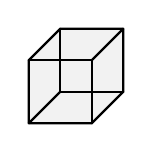
\begin{tikzpicture}[line width=1.3pt, line cap=round, line join=round, >=Stealth, x=1mm,y=1mm]
  \draw[thick, fill=gray!10] (-6,-8) -- (2,-8) -- (6,-4) -- (6,4) -- (-2,4) -- (-6,0) -- cycle;
  \draw[thick] (-6,0) -- (2,0) -- (2,-8);
  \draw[thick] (2,0) -- (6,4);
  \draw[thick] (-2,-4) -- (-6,-8);
  \draw[thick] (-2,-4) -- (-2,4);
  \draw[thick] (-2,-4) -- (6,-4);
\end{tikzpicture}
\end{document}
